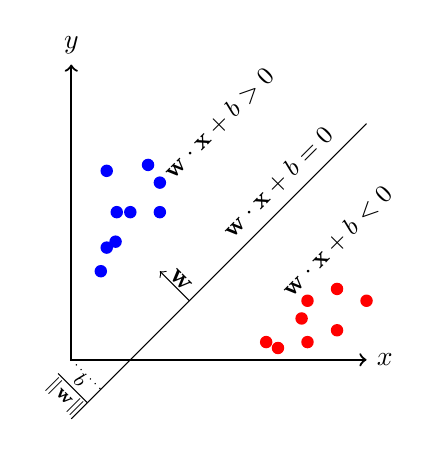
\begin{tikzpicture}[scale=0.75]
  % Draw axes
  \draw [<->,thick] (0,5) node (yaxis) [above] {$y$}
        |- (5,0) node (xaxis) [right] {$x$};
  % Draw line
  \draw (0,-1) -- (5,4); % y=x-1
%  \draw[dashed] (-1,0) -- (4,5); % y=x+1
%  \draw[dashed] (2,-1) -- (6,3); % y=x-3
  % \Draw labels
  \draw (3.5,3) node[rotate=45,font=\small] 
        {$\mathbf{w}\cdot \mathbf{x} + b = 0$};
  \draw (2.5,4) node[rotate=45,font=\small] 
        {$\mathbf{w}\cdot \mathbf{x} + b > 0$};
  \draw (4.5,2) node[rotate=45,font=\small] 
        {$\mathbf{w}\cdot \mathbf{x} + b < 0$};
  % \Draw distance
%  \draw[dotted] (4,5) -- (6,3);
%  \draw (5.25,4.25) node[rotate=-45] {$\frac{2}{\Vert \mathbf{w} \Vert}$};
  \draw[dotted] (0,0) -- (0.5,-0.5);
  \draw (0,-0.5) node[rotate=-45] {$\frac{b}{\Vert \mathbf{w} \Vert}$};
  \draw[->] (2,1) -- (1.5,1.5);
  \draw (1.85,1.35) node[rotate=-45] {$\mathbf{w}$};
  % \Draw negative dots
  \fill[blue] (0.5,1.5) circle (3pt);
  \fill[blue]   (1.5,2.5)   circle (3pt);
  \fill[blue] (1,2.5)     circle (3pt);
  \fill[blue] (0.75,2)    circle (3pt);
  \fill[blue] (0.6,1.9)   circle (3pt);
  \fill[blue] (0.77, 2.5) circle (3pt);
  \fill[blue] (1.5,3)     circle (3pt);
  \fill[blue] (1.3,3.3)   circle (3pt);
  \fill[blue] (0.6,3.2)   circle (3pt);
  % \fill positive dots
  \fill[red] (4,1)     circle (3pt); 
  \fill[red] (3.3,.3)  circle (3pt); 
  \fill[red]     (4.5,1.2) circle (3pt); 
  \fill[red]     (4.5,.5)  circle (3pt); 
  \fill[red]     (3.9,.7)  circle (3pt); 
  \fill[red]     (5,1)     circle (3pt); 
  \fill[red]     (3.5,.2)  circle (3pt); 
  \fill[red]     (4,.3)    circle (3pt); 
\end{tikzpicture}
